\documentclass{article}
\usepackage[a4paper, margin=2cm]{geometry} % <-- Adiciona esta linha
\usepackage{graphicx} % Required for inserting images
\usepackage{amsmath}
\usepackage{float} % For [H] float placement

\title{Séries temporais}
\author{Mariana Fernandes Rocha}
\date{September 2025}

\begin{document}


\begin{titlepage}
    \begin{center}

        \vspace{1cm}
        \begin{minipage}{0.45\textwidth}
            \centering
            
\includegraphics[width=1.2\textwidth]{images/logo_fgv.png}    
        \end{minipage}
        \vspace{2cm}

        \rule{1\textwidth}{0.4pt} \\ % Linha horizontal personalizada
        \vspace{0.2cm}
        {\Huge \textbf{Análise de Séries Temporais}} \\
        \vspace{0.2cm}
        \vspace{0.5cm}
        {\Large \textbf{A1 - Séries Temporais}}\\
        \rule{1\textwidth}{0.4pt} % Linha horizontal personalizada


        \vspace{0.5cm}
        {\Large \textbf{FGV EMAp}} \\
        \vspace{2cm}
        
        

        
        
        % % Unidade e curso
        % {\Large \textbf{FGV EMAp}}\\[2cm]
        
        % Autores
        {\large 
            \textbf{Ana Júlia Amaro Pereira Rocha} \\ 
            \textbf{Henrique Borges Carvalho} \\
            \textbf{Maria Eduarda Mesquita Magalhães}\\
            \textbf{Mariana Fernandes Rocha} \\
            \textbf{Paula Eduarda de Lima}}\\[1.5cm]
        
        % Informações adicionais
        {\large 
            Ciência de Dados e Inteligência Artificial \\ 
            6º Período}\\[2cm]
        
         % Data
        \vfill
        {\large Rio de Janeiro, 2025}

        
    \end{center}
\end{titlepage}

\section*{Discussão sobre métricas e métodos de avaliação}

Para previsões pontuais temos dois grupos de métricas e avaliação: métricas percentuais e métricas absolutas.

Métricas percentuais são adequadas para cenários em que os valores devem ter ordem de grandeza consistente, e mais importante assumir valores distantes de zero, evitando distorções. 

Em uma primeira análise, observa-se que mais de um terço dos dados está no intervalo sujeito a distorções. O intervalo total dos valores é $[0.14, 16.59]$. No entanto, como esses dados potenicialmente distorcidos concentram-se apenas no início e reservamos o final da série para previsões fora do treino, essa limitação, que normalmente inviabilizaria o uso de métricas percentuais, não compromete a análise e tais métricas serão usadas ao longo da análise.


\begin{figure}[h]
    \centering
    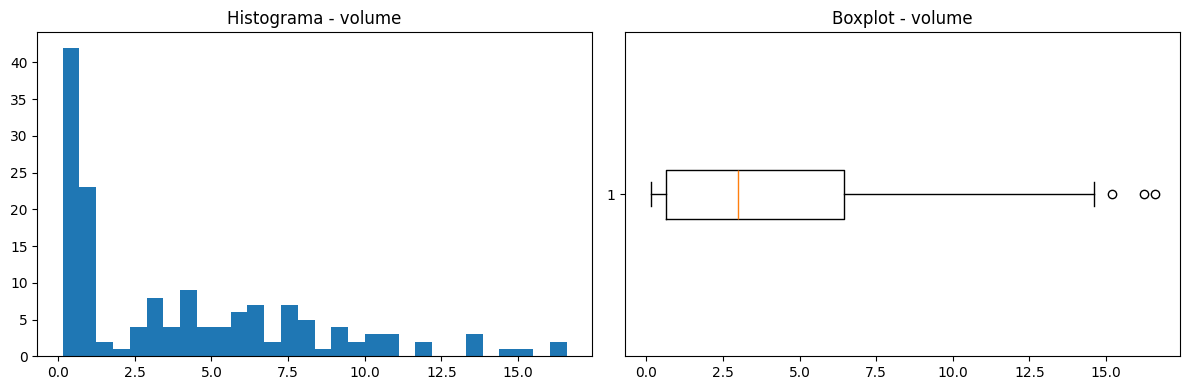
\includegraphics[width=0.75\linewidth]{images/histogram.png}
    \caption{Histograma e distribuição dos valores}
    % \label{fig:placeholder}
\end{figure}

Ademais, serão usadas métricas absolutas que preservam a escala original dos dados, permitindo comparar diretamente as diferenças entre valores observados e previstos. Essa escolha facilita a interpretação dos resultados, mantendo a coerência com a unidade de medida da variável analisada.

Embora o foco até aqui tenha sido a avaliação de previsões pontuais, também serão abordadas previsões distribucionais, o ponto mais importante dessa avaliação é incorporar a incerteza associada às estimativas.
Para isso, derivamos distribuições preditivas a partir da análise dos resíduos dos modelos, assumindo que seguem uma distribuição normal. Essa abordagem possibilita a construção de intervalos de predição e a utilização de métricas específicas para avaliação probabilística, como o CRPS e o Winkler Score.
<<<<<<< HEAD

\section*{Discussão sobre a necessidade de transformação de variáveis}

A série apresentada exibe um comportamento \textbf{claramente crescente ao longo do tempo}, com oscilações cada vez mais amplas a partir de 2024. Esse padrão indica a presença de \textbf{heterocedasticidade}, ou seja, a variância dos valores não é constante — tende a aumentar conforme o nível da série se eleva. Essa característica é comum em séries com crescimento de natureza exponencial ou multiplicativa, e pode comprometer o desempenho de modelos que assumem variância constante.

Nesses casos, é recomendada a aplicação de uma \textbf{transformação de variáveis}, especialmente a \textit{transformação logarítmica} ou a \textbf{transformação de Box-Cox}.  
Usamos a transformação logarítmica cujos efeitos benéficos são:

\begin{itemize}
    \item \textbf{Estabiliza a variância} — reduzindo as oscilações relativas nos períodos de maior valor;
    \item \textbf{Diminui a assimetria da distribuição} dos dados, aproximando-a de uma forma mais normal;
    \item \textbf{Facilita a identificação de padrões estruturais} como tendência e sazonalidade;
    \item \textbf{Torna a relação entre componentes mais aditiva}, melhorando o ajuste de modelos lineares como ARIMA, ETS ou regressão temporal.
\end{itemize}

No caso da série de volume semanal, a transformação é fundamental para corrigir o comportamento multiplicativo observado, permitindo uma análise mais robusta e previsões mais consistentes.

\vspace{1em}

\section*{Discussão sobre a decomposição entre tendência e sazonalidade}

A série apresenta \textbf{um padrão de tendência crescente} e \textbf{flutuações sazonais bem definidas}, com picos e vales que se repetem em intervalos semelhantes. Esse comportamento indica a presença de dois componentes estruturais importantes: a \textbf{tendência de longo prazo} ($T_t$) e a \textbf{sazonalidade periódica} ($S_t$). Assim, a série pode ser representada por:
\[
y_t = T_t + S_t + R_t
\]
onde $R_t$ é o componente residual ou ruído.

A \textbf{decomposição dessa série temporal} é necessária para:

\begin{itemize}
    \item \textbf{Isolar a tendência estrutural}, revelando o crescimento sustentado do volume ao longo do tempo;
    \item \textbf{Identificar padrões sazonais}, observando períodos recorrentes de alta e baixa que podem estar relacionados a ciclos semanais, mensais ou anuais;
    \item \textbf{Remover o efeito da sazonalidade} para ajustar modelos de previsão que dependem de uma estrutura estacionária;
    \item \textbf{Analisar o componente residual}, que expressa as variações aleatórias não explicadas pelos outros fatores.
\end{itemize}

Após a decomposição, a série ajustada sazonalmente mostrou-se muito semelhante à série original o que indica que a tendência sobrepõe a sazonalidade na série temporal em questão, há pouca ou nenhuma sazonalidade.

\begin{figure}[h!]
    \centering
    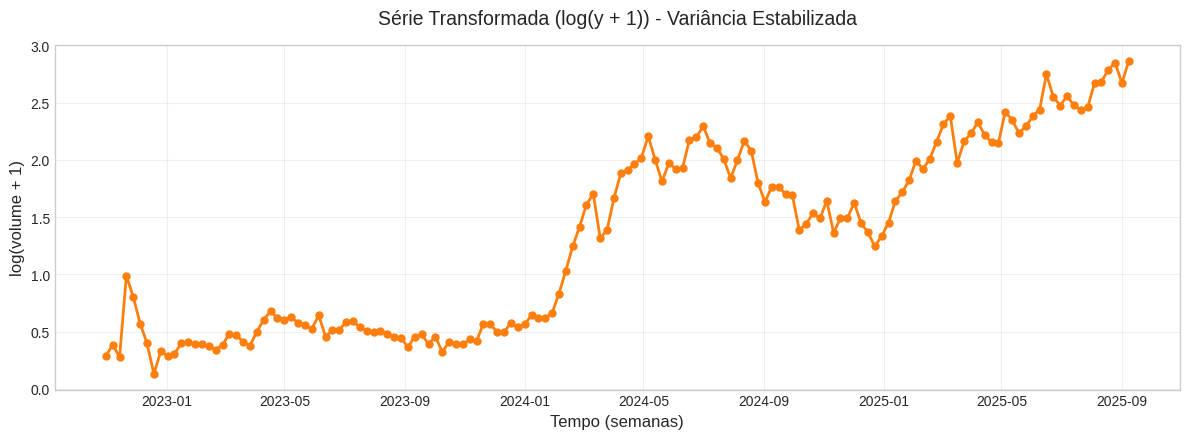
\includegraphics[width=0.75\textwidth]{images/serie_transformada.png}
    \label{fig:serie-transformada}

    \centering
    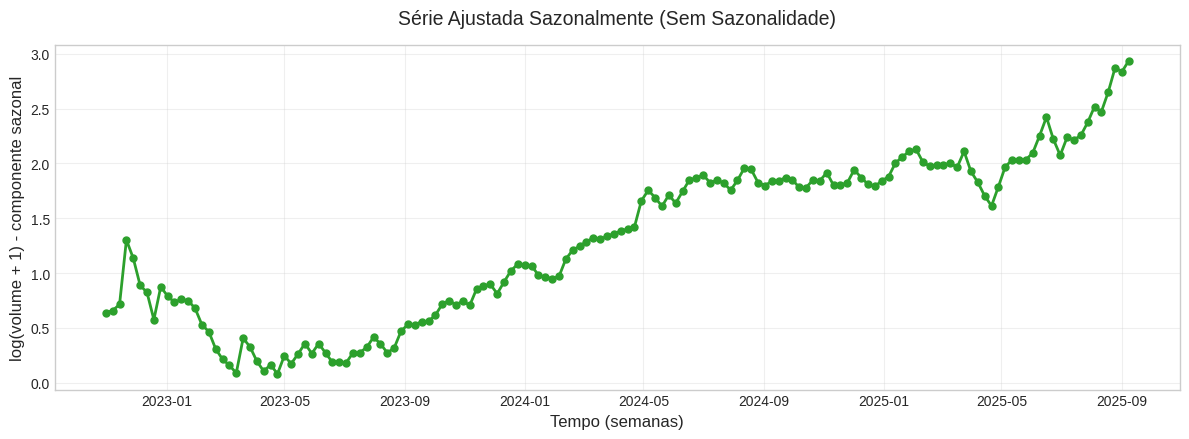
\includegraphics[width=0.75\textwidth]{images/serie_ajustada_sazonalmente.png}
    \label{fig:serie-ajustada-sazonalmente}
\end{figure}

\vspace{1em}

\section*{Análises de resíduos e ajuste dos modelos}

Criamos uma classe chamada \texttt{ResidualAnalysis} que implementa uma análise completa e sistemática de resíduos para modelos de séries temporais, utilizando uma abordagem estatística rigorosa para avaliar a qualidade dos modelos preditivos. O código realiza três tipos principais de análise: testes estatísticos formais, análise gráfica abrangente e diagnóstico comparativo entre modelos.

A análise inicia com testes estatísticos formais que avaliam quatro pressupostos fundamentais: normalidade dos resíduos (teste Anderson-Darling), ausência de autocorrelação (Ljung-Box e Durbin-Watson), homocedasticidade (teste ARCH) e média zero (teste t). Paralelamente, são gerados 12 gráficos diagnósticos que permitem a visualização multidimensional dos resíduos, incluindo ACF/PACF, Q-Q plots, resíduos versus valores ajustados, e distribuições comparativas.

Baseado nas análises que fizemos, podemos observar uma hierarquia clara na qualidade dos modelos:

\begin{itemize}
    \item \textbf{SARIMAX}: Melhor desempenho geral (pontuação: 1.998) com RMSE mais baixo (0.675)
    \item \textbf{Regression}: Performance intermediária (pontuação: 0.000) com RMSE moderado (1.404)
    \item \textbf{Modelos de baseline}: Performance inferior com RMSE elevado (6.300-10.606)
\end{itemize}

O SARIMAX destacou-se por atender aos critérios de ausência de autocorrelação e média zero, embora apresente problemas de normalidade e heterocedasticidade. 

Apesar do bom desempenho do SARIMAX, a falha no teste de normalidade sugere que transformações nos dados ou ajustes na especificação do modelo podem melhorar ainda mais sua performance. Para o modelo de Regression, a presença de autocorrelação indica a necessidade de incorporar componentes autorregressivos ou usar erros padrão robustos.

A análise comparativa demonstra que modelos mais sofisticados que incorporam estrutura temporal (SARIMAX) superam significativamente tanto modelos de regressão convencionais quanto abordagens de baseline, destacando a importância de considerar a dependência temporal na modelagem. As análises completas dos outros modelos podem ser verificadas no arquivo ipynb.

\begin{figure}[H]
    \centering
    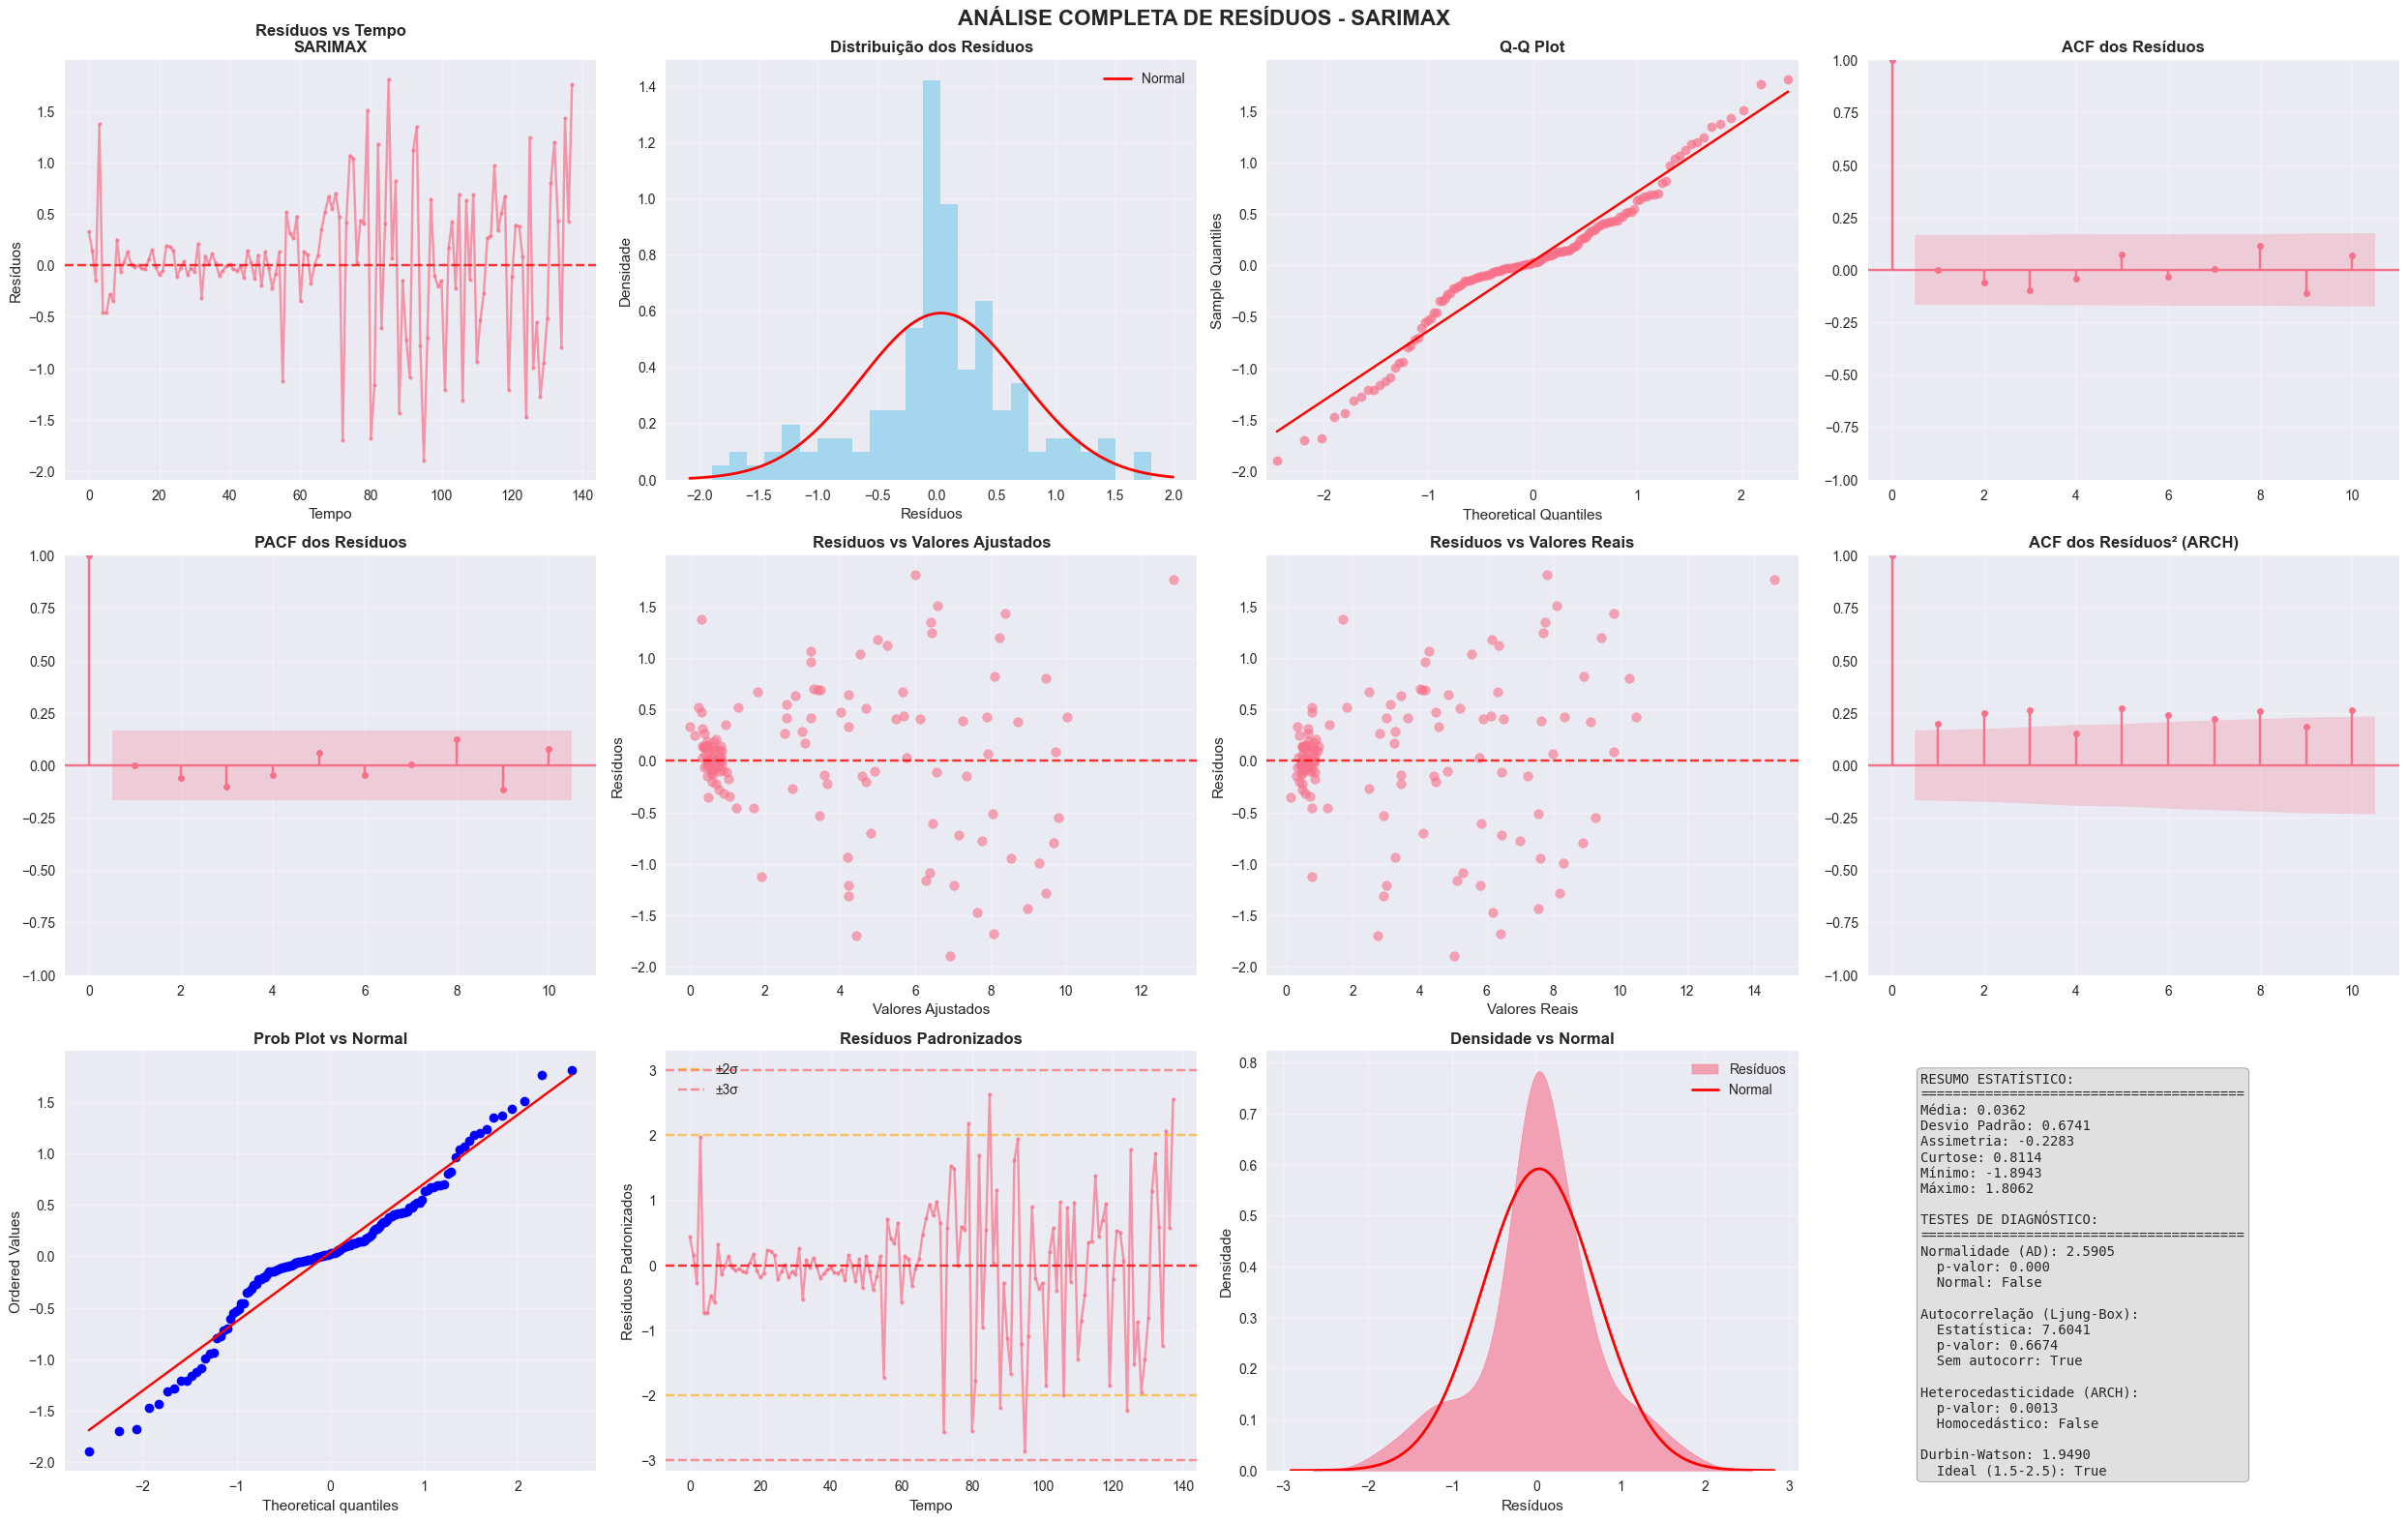
\includegraphics[width=0.9\textwidth]{images/sarimax_analisado.png}
    \caption{Análise completa de resíduos do modelo SARIMAX}
    \label{fig:sarimax_residuals}
\end{figure}



\section*{Modelos baselines}

Modelos baseline são abordagens de previsão simples que servem como um ponto de referência para avaliar o desempenho de modelos mais complexos. A sua principal função é estabelecer um limiar de performance: se um modelo sofisticado não conseguir superar um baseline simples, isso sugere que o modelo mais complexo não está capturando bem os padrões da série ou que a série é inerentemente difícil de prever. Para este trabalho, foram implementados cinco modelos baseline, cujos resultados foram comparados utilizando as métricas MAE, RMSE e MAPE.

\subsection*{Mean Method}
Este é o baseline mais simples, onde a previsão para qualquer período futuro é a média de todos os valores observados no conjunto de treino.
$$ \hat{y}_{T+h|T} = \bar{y} = \frac{1}{T}\sum_{t=1}^{T}y_t $$

\subsection*{Naive Method}
Neste método, a previsão para o próximo período é simplesmente o último valor observado.
$$ \hat{y}_{T+h|T} = y_T $$

\subsection*{Seasonal Naive}
Uma variação do Naive Method, útil para séries com forte sazonalidade. Ele prevê o valor futuro utilizando a observação do mesmo período no ciclo sazonal anterior. Utilizamos dados semanis considerando sazonalidade anual, o período é $m=52$.
$$ \hat{y}_{T+h|T} = y_{T+h-m} $$

\subsection*{Drift Method}
Este método é uma extensão do Naive e é adequado para séries com tendência. Ele extrapola uma linha traçada entre a primeira e a última observação do conjunto de treino. A previsão incorpora uma "inclinação" (drift) média.
$$ \hat{y}_{T+h|T} = y_T + h \left( \frac{y_T - y_1}{T-1} \right) $$

\subsection*{Média Móvel}
A previsão é calculada como a média dos últimos $K$ valores observados no conjunto de treino. Este método suaviza flutuações de curto prazo. Para este estudo, foi utilizado $K=4$.
$$ \hat{y}_{T+h|T} = \frac{1}{K}\sum_{t=T-K+1}^{T}y_t $$

\subsection*{Resultados e Análise}
Os modelos foram treinados com os primeiros 120 pontos da série e avaliados nos 30 pontos subsequentes. Os resultados obtidos para as métricas de erro no conjunto de teste estão consolidados na Tabela 1.

\begin{table}[h]
    \centering
    \begin{tabular}{|l|c|c|c|}
        \hline
        \textbf{Modelo} & \textbf{MAE} & \textbf{RMSE} & \textbf{MAPE (\%)} \\
        \hline
        Drift & 3.9666 & 4.6585 & 34.40 \\
        Seasonal Naive & 4.7593 & 5.4027 & 44.01 \\
        Naive & 4.6803 & 5.4411 & 40.79 \\
        Média móvel (k=4) & 5.0153 & 5.7318 & 44.20 \\
        Mean & 7.9639 & 8.4335 & 74.25 \\
        \hline
    \end{tabular}
    \caption{Resultados dos Modelos Baseline no Conjunto de Teste.}
    \label{tab:baseline_results}
\end{table}

Analisando a Tabela \ref{tab:baseline_results}, o \textbf{Drift Mathod} apresentou o melhor desempenho em todas as métricas, com um RMSE de 4.6585. Isso sugere que a série possui uma componente de tendência linear que é capturada de forma eficaz por este método. Os modelos Naive e Seasonal Naive tiveram performances intermediárias e muito similares, indicando que tanto a dependência do último ponto quanto a sazonalidade anual são características relevantes, mas secundárias à tendência geral. O Mean Method foi o que obteve o pior resultado, o que era esperado para uma série não estacionária com tendência.

O desempenho do modelo de Drift estabelece, portanto, o principal benchmark a ser superado pelos modelos mais complexos que serão analisados nas próximas seções.

\section*{Modelos de Regressão}

Foi realizada uma análise completa de séries temporais utilizando dois enfoques principais: \textbf{Regressão Linear Múltipla (OLS)} e \textbf{modelos SARIMAX}. O objetivo geral foi capturar componentes de tendência, sazonalidade e autocorrelação, além de comparar o desempenho preditivo entre os modelos.

\subsection*{Regressão Linear Múltipla (OLS)}
O modelo OLS considerou a variável dependente \texttt{volume}, com preditores que representam a tendência temporal (\texttt{t}), harmônicos sazonais (\texttt{sin1}, \texttt{cos1}, \texttt{sin2}, \texttt{cos2}) e dummies mensais (\texttt{m\_2} a \texttt{m\_12}).  
O objetivo foi ajustar um modelo interpretável capaz de representar tendência e sazonalidade. O diagnóstico de resíduos incluiu ACF/PACF, histograma, QQ-Plot e teste de Ljung-Box. As métricas de desempenho utilizadas foram \textbf{RMSE} e \textbf{MAPE}, calculadas sobre o conjunto de teste (últimas 12 semanas). Como veremos mais a frente, na análise de resíduos, o modelo OLS não capturou adequadamente a estrutura dos dados.

\begin{table}[h!]
\centering
% \caption{Resultados da Regressão OLS}
\begin{tabular}{ll}
\hline
\textbf{Variável} & \textbf{Valor} \\
\hline
Dep. Variable       & volume \\
No. Observations    & 150 \\
Df Residuals        & 133 \\
Df Model            & 16 \\
R-squared           & 0.806 \\
Adj. R-squared      & 0.783 \\
F-statistic         & 34.61 \\
Prob (F-statistic)  & 1.50e-39 \\
AIC                 & 632.3 \\
BIC                 & 683.5 \\
\hline
\end{tabular}
\end{table}

\subsection*{Modelos SARIMAX}
Como os resultados do OLS não se mostraram promissores, pesquisamos outros modelos de regressão mais robustos que pudessem melhorar o desempenho nesses dados. Os modelos SARIMAX foram empregados para capturar dependências temporais não explicadas pela regressão, incluindo componentes autorregressivos (AR), de média móvel (MA) e sazonais (P, D, Q, m).  
A seleção de parâmetros foi realizada via \texttt{auto\_arima} e grid search manual. Foram aplicados os mesmos diagnósticos de resíduos e métricas de avaliação (RMSE, MAPE), além de critérios de informação \textbf{AIC} e \textbf{BIC}. O melhor resultado foi
o SARIMAX (0,1,1) x (0,1,1,52) (AIC=83.05, BIC=87.36)

\subsection*{Comparação e Resultados}
Os resultados comparativos mostraram que o modelo OLS não o  capturou adequadamente a estrutura dos dados e tenho um erro maior, enquanto o SARIMAX apresenta melhor ajuste em termos de dependência temporal e critérios de informação, como podemos ver pelo gráfico e pelos erros comparados.  

\begin{table}[h]
    \centering
    \begin{tabular}{|l|c|c|c|}
        \hline
        \textbf{Modelo}  & \textbf{RMSE} & \textbf{MAPE (\%)} \\
        \hline
        OLS & 5.1834 & 0.3303 \\
        SARIMAX  & 3.2793 & 0.2212 \\
        \hline
    \end{tabular}
    % \caption{Resultados dos Modelos de regressão no Conjunto de Teste.}
    \label{tab:baseline_results}
\end{table}

\begin{figure}[h]
    \centering
    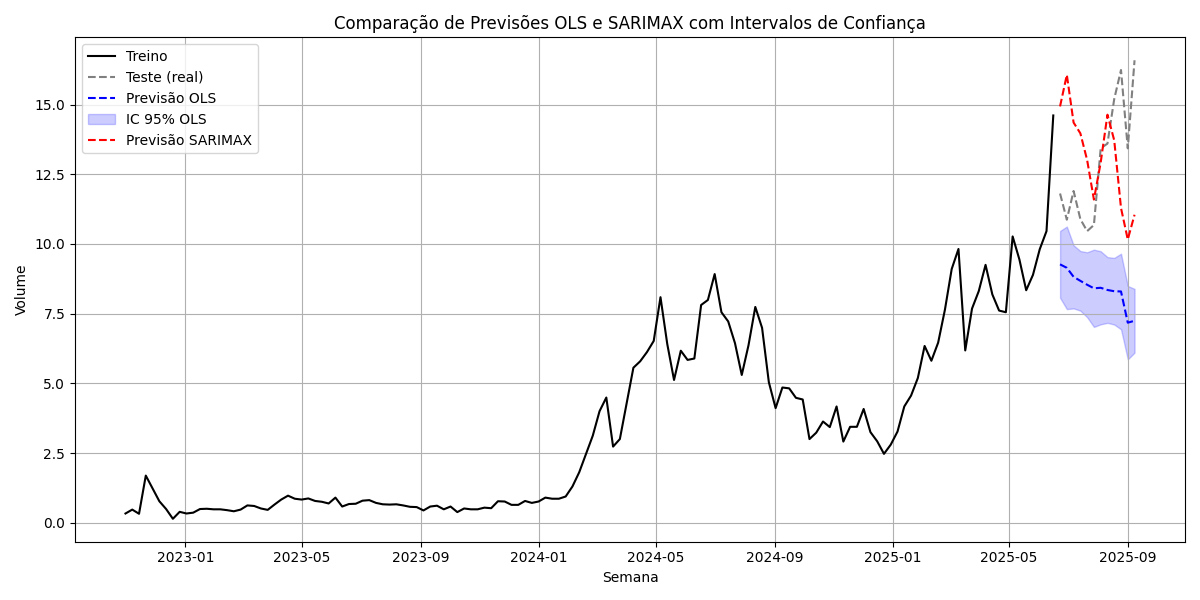
\includegraphics[width=0.75\linewidth]{images/forecast_comparison.png}
    % \caption{Histograma e distribuição dos valores}
    % \label{fig:placeholder}
\end{figure}





\end{document}